\documentclass{article}
\usepackage[utf8]{inputenc}
\usepackage[english]{babel}
\usepackage{graphicx}
\usepackage{float}
\usepackage{listings}
\usepackage{hyperref}
\usepackage{amsmath}
\hypersetup{
    colorlinks=true,
    linkcolor=blue,
    filecolor=magenta,      
    urlcolor=cyan,
}
\urlstyle{same}

\title{Manual 3 - 2do Torneo de Programación Competitiva}
\author{Lions R.C.}
\date{Julio 2019}

\begin{document}

\maketitle

\tableofcontents

\begin{figure}[H]
    \centering
    
\includegraphics[width=0.2\paperwidth]{newblack}
\end{figure}

\section{Estructuras de datos avanzadas}

Hasta ahorita solo hemos visto estructuras de datos sencillas (vectores, pares, mapas y sets) que tienen el proposito de guardar valores de una manera conveniente para su acceso. Ahora se verán estructuras que guardan valores en cierta orden o configuración con el fin de simplificar programas más avanzadas.

\subsection{Stack}

El stack o la pila en español es una estructura de datos que, como indica su nombre, apila datos desde abajo hasta arriba. El concepto detrás de esta estructura es igual al de la vida real; si tienes una caja donde vas apilando hojas, debes sacar la hoja que esta hasta arriba antes de que puedas sacar la que esta debajo de esa y viceversa.

Digamos que tenemos 6 enteros, {6, 5, 2, 9, 3} y los insertamos en nuestra pila empezando con 6 y terminando con 3. Nuestra pila se verá de la siguiente manera:

\begin{figure}[H]
    \centering
    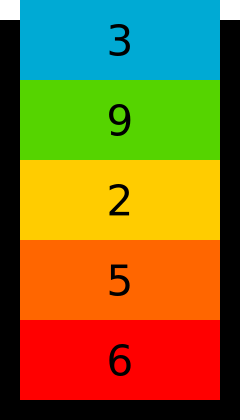
\includegraphics[width=0.1\paperwidth]{pila}
\end{figure}

Debido a la implementación interna de la pila, no podemos sacar un valor que este debajo de otro sin sacar todos los de arriba primero. Esta propiedad se llama \textbf{LIFO} en íngles o Last In First Out (el último en entrar es el primero en salir).

Si ahora sacamos todos los valores y los guardamos en un arreglo, veremos que se invertió el orden de los datos debido a esta propiedad: {3, 9, 2, 5, 6}.

Para incluir una pila en C++, se llama la librería \textbf{stack} y se declara con sintaxis \textbf{\lstinline{stack<tipo> nombre;}}.

Para agregar objetos a una pila, se puede utilizar la función \textbf{push(valor)} y para eliminar el dato que esta hasta arriba se debe hacer \textbf{pop()}. Para ver el dato que esta hasta arriba se puede utilizar \textbf{top()} y para ver cuantos elementos tiene se puede llamar a \textbf{size()}.

Vamos a crear un programa que invierte los valores que originalmente habiamos visto:

\begin{lstlisting}[language=C++, caption=Pilas]
#include <iostream>
#include <stack>

using namespace std;

int main() {
    stack<int> pila;
    int valores[] = {6, 5, 2, 9, 3};
    for(int i = 0; i < 5; i++) {
        pila.push(valores[i]);
    }
    while(pila.size() > 0) {
        cout << pila.top() << endl;
        pila.pop();
    }
}
\end{lstlisting}
\href{https://repl.it/@Jamesscn/Cargando-pilas}{Liga al código} \\

Como se puede observar al correr el programa, los valores se imprimen al revés.

La pila no solo sirve para invertir cosas, sino que es util para cuando quieres procesar los datos más recientes antes que las más antiguas.

Digamos que estas diseñando el buzón de un red social como Facebook o Twitter y tu quieres enseñarle a tus usuarios las publicaciones más recientes, pero también quieres eliminar las publicaciones vistas por el usuario para que no tengan que desplazarse mucho para ver más contenido.

Esto se puede implementar con una pila que va apilando las publicaciones más recientes y cada vez que el usuario se desplaza para abajo se quitan las publicaciones que estan hasta arriba.

\subsection{Queue}

El queue o la fila es en cierto sentido el complemento de la pila. La fila, como también indica el nombre, funciona como una fila de datos donde el primero en entrar es el primero en salir. Esto se llama \textbf{FIFO} en íngles o First In First Out.

\begin{figure}[H]
    \centering
    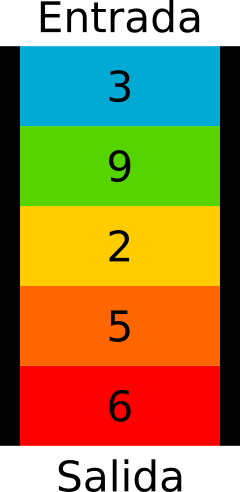
\includegraphics[width=0.1\paperwidth]{fila}
\end{figure}

Como se puede observar, los datos estan haciendo fila y saldrían en el mismo orden de la que entran, no se invierten. Al igual que una pila, un valor que esta hasta atrás no puede salir primero.

Para implementarlo, se debe incluir la librería \textbf{queue} y se debe declarar como \textbf{\lstinline{queue<dato> nombre;}}.

Las funciones de esta estructura son algo distintos a las de la pila. Para insertar y quitar datos, se puede utilizar \textbf{push(valor)} y \textbf{pop()} respectivamente, pero para ver el valor que esta hasta en frente se debe llamar \textbf{front()}. Como támbien tiene una parte de atrás, este se puede ver con \textbf{back()}.

\begin{lstlisting}[language=C++, caption=Filas]
#include <iostream>
#include <queue>

using namespace std;

int main() {
    queue<int> fila;
    int valores[] = {6, 5, 2, 9, 3};
    for(int i = 0; i < 5; i++) {
        fila.push(valores[i]);
    }
    while(fila.size() > 0) {
        cout << fila.front() << endl;
        fila.pop();
    }
}
\end{lstlisting}
\href{https://repl.it/@Jamesscn/Haciendo-filas}{Liga al código} \\

Esta estructura es bastante útil debido a que ahorra memoria al borrar datos que ya no ocupa y permite hacer una especie de buffer o vector que almacena datos que no se pueden procesar uno por uno.

Un ejemplo de la fila es cuando quieres promover un producto tuyo a muchas personas. Puedes empezar promoviendole a un amigo tuyo y preguntandole si tiene amigos que le interesa tu producto, luego preguntas a cada uno de esos amigos por sus amigos y sigues repitiendo el proceso hasta haber promovido tu producto a una cantidad satisfactoria de gente.

La pila junto con la fila se aplicarán en las semanas que siguen para resolver problemas relacionados a grafos, como encontrar la respuesta a un laberinto o averiguar el camino más rápido entre dos ciudades.

\subsection{Deque}

El deque es una estructura especial debido a que puede funcionar como pila y fila a la vez. El nombre deque viene del termino double ended queue en íngles o fila con dos salidas.

Se llama de esta manera debido a que funciona como una pila porque puedes insertar datos y luego sacar el primer dato que fue ingresado, y además puedes sacar el último dato que fue ingresado.

\begin{figure}[H]
    \centering
    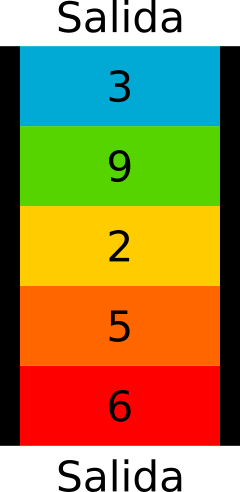
\includegraphics[width=0.1\paperwidth]{deque}
\end{figure}

Si usamos este ejemplo, no podemos obtener los valores de en medio, pero sí podemos sacar el 3 o el 6. Si quitamos el 3, ahora podríamos quitar el 9 o el 6.

Para implementar un deque, se debe incluir la librería \textbf{deque} y se puede crear con \textbf{\lstinline{deque<tipo> nombre;}}

El deque fue implementado de una manera más flexible que las otras estructuras, y sí te permite ver los datos que están en su interior. Para guardar un dato en la parte de enfrente o quitar un dato, se pueden usar \textbf{\lstinline{push_front(valor)}} y \textbf{\lstinline{pop_front(valor)}} respectivamente, y para guardar datos en la parte de atrás de debe llamar \textbf{\lstinline{push_back(valor)}} y \textbf{\lstinline{pop_back()}}.

Se debe notar que el valor en frente es la que se encuentra en la posición 0 y el valor de atrás es la que está en la posición $N - 1$.

Para ver o modificar algún valor se puede usar el sintaxis de un arreglo, como \textbf{nombre[índice]}. Para ver el valor que esta hasta enfrente o hasta atrás, es recomendable utilizar \textbf{front()} y \textbf{back()}. Para insertar o eliminar valores existen las funciones \textbf{insert()} y \textbf{erase()}.

Un ejemplo práctico del deque es para determinar si una palabra es palindromo. Se puede insertar la palabra en el deque y luego se puede comparar el carácter de enfrente con el de atrás e irlos sacando de dos en dos hasta que quede cero o un valor en el deque.

\begin{lstlisting}[language=C++, caption=Deques]
#include <iostream>
#include <deque>

using namespace std;

int main() {
    string palindromo = "aibofobia";
    deque<char> dobleFila;
    //insertar a la fila
    for(int i = 0; i < palindromo.length(); i++) {
        dobleFila.push_back(palindromo[i]);
    }
    bool valido = true;
    while(dobleFila.size() > 1) {
        if(dobleFila.front() != dobleFila.back()) {
            valido = false;
            break;
        }
        dobleFila.pop_front();
        dobleFila.pop_back();
    }
    if(valido) {
        cout << palindromo << " es un palindromo" << endl;
    } else {
        cout << palindromo << " no es un palindromo" << endl;
    }
}
\end{lstlisting}
\href{https://repl.it/@Jamesscn/Deque}{Liga al código}

\subsection{Priority queue}

El priority queue es una especie de fila con prioridad como indica el nombre. Este guarda los valores como una fila normal, pero el primero en salir siempre será el valor mas grande en la fila.

Por ejemplo, un hospital usaría una fila de prioridad para atender sus pacientes, atendiendo al paciente más urgente primero.

Para usar este tipo de dato, se incluye la librería \textbf{queue} igual que cuando se estaba usando una fila y se declara con \textbf{\lstinline{priority_queue<tipo> nombre;}}

Las funciones de este tipo son \textbf{push(valor)} y \textbf{pop()} para agregar o quitar valores y \textbf{top()} para ver el valor que esta enfrente de la fila.

Un ejemplo de estos sería un programa que ordena un arreglo de números flotantes.

\begin{lstlisting}[language=C++, caption=Filas de prioridad]
#include <iostream>
#include <queue>

using namespace std;

int main() {
    float valores[] = {2.22, 3.56, 1.9, 9.52, 3.42, 6.78, 0.11, 4.5};
    priority_queue<float> fila;
    for(int i = 0; i < 8; i++) {
        fila.push(valores[i]);
    }
    for(int i = 0; i < 8; i++) {
        cout << fila.top() << endl;
        fila.pop();
    }
}
\end{lstlisting}
\href{https://repl.it/@Jamesscn/Prioridades}{Liga al código}

Esta estructura es muy parecida a un heap, que guarda el dato más grande sobre los demás valores.

\section{Recursividad}

\subsection{Factoriales}

\subsection{Series de Fibonacci}

\section{Programación dinámica}

\subsection{Series de Fibonacci}

\end{document}